\section{Comparison}

\begin{figure}[H]
    \centering
    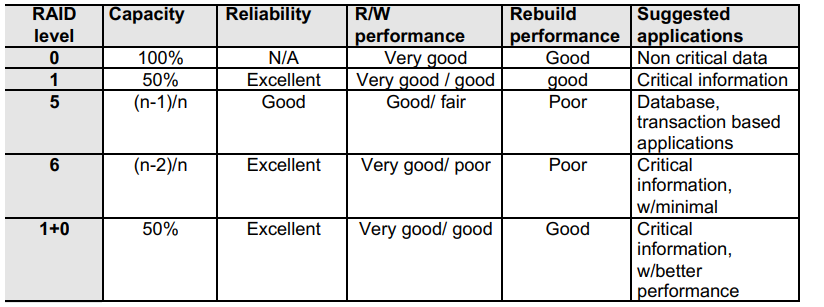
\includegraphics[width=0.6\linewidth]{images/levchar.png}
    \caption{RAID levels characteristics}
\end{figure}
Based on the context information provided, the best performance and most capacity can be achieved with RAID 0. 
This is because RAID 0 allows for the striping of data across multiple drives, which can significantly increase read and write speeds. 
However, it is important to note that RAID 0 does not provide any data redundancy or fault tolerance, so it is not recommended for use in critical data storage scenarios.

The greatest error recovery can be achieved with RAID 1 (1+0 or 0+1). This is because RAID 1 provides data redundancy by mirroring data across multiple drives. 
If one drive fails, the data can still be accessed from the other drives. 
However, it is important to note that RAID 1 can also result in a decrease in performance compared to RAID 0.

The balance between space, performance, and recoverability can be achieved with RAID 5. 
This is because RAID 5 provides a balance between the three by allowing for data striping across multiple drives while also providing some level of data redundancy. 
However, it is important to note that RAID 5 can also result in a decrease in performance compared to RAID 0.

\subsection{Hot spares}
Many RAID systems include a hot spare, which is an idle, unused disk installed in the system.
In the event of a drive failure, the array is immediately rebuilt using the hot spare, allowing for seamless data recovery and minimizing downtime.

\subsection{Implementation}
RAID is a data storage technology that allows multiple hard drives or solid-state drives to be combined into a single logical unit that can be accessed as if it were a single drive. 
RAID can be implemented in either hardware or software.

Hardware RAID is implemented using specialized hardware controllers that are built into the motherboard or a separate expansion card. 
Hardware RAID is generally faster and more reliable than software RAID, as it offloads the processing of managing the RAID array to dedicated hardware. 
However, migrating a hardware RAID array to a different hardware controller can be challenging and may not always work successfully.

On the other hand, software RAID is implemented using software drivers that run on the computer's central processing unit (CPU). 
Software RAID is simpler to migrate and cheaper than hardware RAID, but it has worse performance and weaker reliability due to the consistent update problem. 
This problem occurs because software RAID relies on the CPU to manage the RAID array, which can cause performance issues if the CPU is not powerful enough or if there are other processes running on the computer that require CPU resources.